\documentclass[a4paper,12pt]{article}

\usepackage{titlesec}
\setcounter{secnumdepth}{4}
\titleformat{\paragraph}
{\normalfont\normalsize\bfseries}{\theparagraph}{1em}{}
\titlespacing*{\paragraph}
{0pt}{3.25ex plus 1ex minus .2ex}{1.5ex plus .2ex}

%% Language and font encodings
\usepackage[english]{babel}
\usepackage[utf8x]{inputenc}
\usepackage[T1]{fontenc}

%% Sets page size and margins
\usepackage[a4paper,top=3cm,bottom=2cm,left=3cm,right=3cm,marginparwidth=1.75cm]{geometry}

%% Useful packages
\usepackage{amsmath}
\usepackage{mathtools}

\usepackage{amssymb}
\usepackage{listings}
\usepackage{fontspec}
\newfontfamily{\braille}{DejaVu Serif}

\usepackage{graphicx}
\usepackage[colorinlistoftodos]{todonotes}
\usepackage[colorlinks=true, allcolors=blue]{hyperref}
\DeclarePairedDelimiter\set\{\}

\title{Efficient Universal Turing machine simulation in $\mathcal{O}(T\log T)$-time\footnotemark}
\author{Kenenbek Arzymatov}
\begin{document}
\maketitle

\section{Introduction}
\subsection{Turing Machine}


\footnotetext{Presentation slides are accessible \href{https://docs.google.com/presentation/d/1NKgTRBZZgML2MXeKdbmro6EjdUyeMWOgLDkzd1AltRQ/edit?usp=sharing}{here}}

\par 
It is possible to think about a Turing Machine (TM) as model of simple computer. Due to its simplicity computer scientists and mathematicians can use it to study the theoretical properties of computation. For instance, they managed to discover that no matter how powerful computer is, it is always achievable to translate its programs to work on the Turing Machine or that all programming languages can do the same things. 

\par
One of the central concepts in compution is "algorithm" because algorithm is a way for solving a particular problem.  
Let $f$ be a function that takes a string of zeros and ones (element of the set
$\{0, 1\}^{∗}$ ), here \textit{star}-operation means: 
$$A^* = \{x_0x_1\dots x_k | k \geq 0 \text{ and each }x_i \in A \}$$
 and outputs either 0 or 1. An algorithm for computing $f$ is a set of mechanical
rules, such that by following them it is possible to compute $f (x)$ given any input $x \in \{0, 1\}^{∗}$ . The
set of rules being followed is fixed (the same rules must work for all possible inputs)
though each rule in this set may be applied arbitrarily many times. Each rule involves
one or more of the following "elementary" operations: 

\begin{itemize}
\item Read a symbol on the inpute tape 
\item Read a symber on the work tape if TM has it 
\item Write a symbol to the work tape 
\item Eiter stop and output 0 or 1, or choose a new rule for the next step.
\end{itemize}

\par 
The \textit{running time} of an algorithm is the number of these basic operations performed. It's
measured in asymptotic terms. For example, if a machine runs in time $T(n)$ then it executes at most $T(n)$ basic operations time on inputs of length $n$. 

\par 
Figure \ref{fig:tm} is an illustration for 3-tape TM with an input, work and output tapes.
\begin{figure}[!ht]
\centering
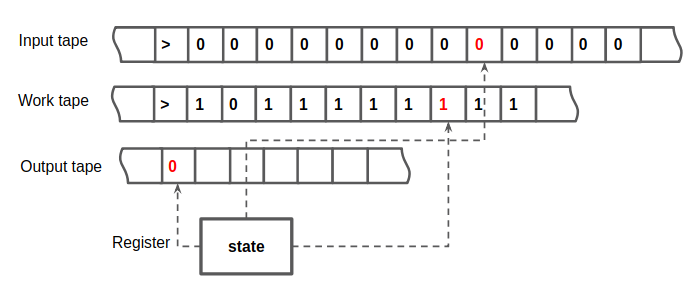
\includegraphics[width=10cm]{tm.png}
\caption{Example of Turing machine with three tapes: an input tape, a work tape and an output tape.}
\label{fig:tm}
\end{figure}


\textbf{Definition}. TM $M$ is described by a tuple $(\Gamma, Q, \delta)$ containing:

\begin{itemize}
\item A finite set  of the symbols that $M$’s tapes can contain. It contains a
designated "blank" symbol, denoted  $\square$; a designated "start" symbol, denoted  $\rhd$; and
the numbers 0 and 1. This set is called the alphabet of TM $M$.
\item A finite set $Q$ of possible states $M$’s register can be in. $Q$ contains a
designated start state, denoted $q_{start}$ , and a designated halting state, denoted $q_{halt}$
\item A function $\delta : Q \times \Gamma^{k} → Q \times \Gamma^{k−1} \times \set*{L, S, R}^{k}$ , where $k \geq 2$, describing the rules $M$
use in performing each step; $L, S, R$ stand for move $L$eft, $S$tay in place or move $R$ight accordingly. This function is called the transition function of $M$.
\end{itemize}

\textbf{Useful statements}:
\begin{enumerate}
\item Behavior of a Turing machine is determined by its transition function. For example,
$\delta(q, (\sigma_1, \dots, \sigma_k)) = (q', \sigma^{'}_2, \dots, \sigma^{'}_k), z) $ where $z \in \{L, S, R\}^{k}$ like $LS\dots SR$ or $RR\dots LS$. For example, if TM has 3 work tapes and output tape $z$ can be like $SRRR$ which means stay in place for the first tape and move heads right for the other ones. 
\item  An algorithm (machine) can be represented as a bit string (consisting only of zeros and ones) by the means of encoding. For example, there is a function which takes an integer number and return an incremented one:
\begin{lstlisting}[language=C]
int function (int x){
   x = x + 1; 
   return x**2; 
}
\end{lstlisting}

The code above can be encoded with Braille font  (just for illustrative purposes only):
{\obeylines\braille
⡂⡀⣀⢀⣄⡀⣰⡉⡀⠀⡀⡀⣀⠀⢀⣀⢀⣄⡀⡂⢀⣀⡀⢀⢀⡀⠀⡰⣀⠀⣀⠀⡂⡀⣀⢀⣄⡰⡀⢠⠂
⡇⡏⠀⡇⡇⠀⢸⠀⡇⢀⡇⡏⠀⡇⣏⠀⠀⡇⠀⡇⣏⠀⣹⢸⠁⢸⠀⡇⢈⠷⡁⠀⡇⡏⠀⡇⡇⠀⡇⢼⠀
⠁⠁⠀⠁⠈⠁⠈⠀⠈⠁⠁⠁⠀⠁⠈⠉⠀⠈⠁⠁⠈⠉⠁⠈⠀⠈⠀⠱⠉⠀⠉⠀⠁⠁⠀⠁⠈⠱⠁⠘⠄⠀⠀⠀⠀⠀⠀⠀⠀⠀⠀⠀⠀⠀⠀⠀⠀⠀⠀⠀⠀⠀⠀⠀⠀⠀⠀⠀
⠀⠀⠀⢤⡀⡤⠀⣀⣀⣀⠀⢤⡀⡤⠀⠀⢰⠀⠀⢹⠀
⠀⠀⠀⣠⠛⣄⠀⠒⠒⠒⠀⣠⠛⣄⠀⠉⢹⠉⠁⢸⠀
⠀⠀⠀⣄⢄⠤⢄⢴⠤⢠⠀⢠⢠⡠⢠⡠⢄⠀⢤⡀⡤⢺⡖⠐⣷⠂⠊⢉⡆
⠀⠀⠀⡇⠸⣍⣉⠸⣀⠸⣀⢼⢸⠀⢸⠀⢸⠀⣠⠛⣄⠀⠀⠀⠀⠀⣴⣋⡀
⠀⠀⠀⠀⠀⠀⠀⠀⠀⠀⠀⠀⠀⠀⠀⠀⠀⠀⠀⠀⠀⠀⠀⠀⠀⠀⠀⠀⠀
⢱⠀
⢸⠁
⠊
}

The result of converting the dots to ones and the blanks to zeros is the bitstring. 

$\underbrace{1000010011001011111001000011111100010001111010 \dots 101001001011010011}_\text{length}$

\item Every string in $\{0, 1\}^{*}$ represents some Turing machine.
\item An algorithm/machine can be used as a possible input
to another algorithm — this makes the boundary between input, software, and hardware
very thin. 
\item Every TM is represented by infinitely many strings.
\item $M_\alpha$ is the TM whose representation as a bit string is $\alpha$. 
\end{enumerate}

\textbf{Definition.} 
Let $f : \{0, 1\}^{∗} \rightarrow \{0, 1\}^{*}$ and let $T :  \mathbb{N} →  \mathbb{N}$ be some functions, and let $M$ be a Turing
machine. We say that $M$ computes $f$ if for every $x \in \{0, 1\}^{*}$ , whenever $M$ is initialized
to the start configuration on input $x$, then it halts with $f(x)$ written on its output tape.
We say $M$ computes $f$ in $T(n)$-time if its computation on every input $x$ requires at most $T(|x|)$ steps.


\subsection{The universal Turing machine}
\textbf{Definition}.There is a universal Turing machine $U$ that can simulate any other Turing machine given
its bit representation. Given a pair of bit strings $(x, \alpha)$ as input, this machine simulates
the behavior of $M_\alpha$ on input x. This simulation is very efficient: If the running time of
$M_\alpha$ was $T(|x|)$, then the running time of $U$ is $O(T(|x|) \log{T(|x|)})$.
Turing was the first to observe that general-purpose computers are possible, by showing
a universal Turing machine that can simulate the execution of every other TM $M$ given
$M$’s description as input.

\par 
Nowadays people who has a programming background easily can understand that the same function can be implemented on any programming language. 
But it is good to remember why it was once counterintuitive. The parameters of the universal
TM are fixed—alphabet size, number of states, and number of tapes. The corresponding
parameters for the machine being simulated could be much larger. The reason this is the ability to use encodings. Even if the universal TM has a
very simple alphabet, this suffices to represent the other machine’s state and transition
table on its tapes and then follow along in the computation step by step.

\subsection{Efficient universal Turing machine}
\textbf{Theorem}.There exists a TM $U$ such that for every $x, \alpha \in \{0, 1\}^{*} , U(x, \alpha) = M_\alpha(x)$, where $M_\alpha$
denotes the TM represented by $\alpha$.
Moreover, if $M_\alpha$ halts on input x within T steps then $U(x, \alpha)$ halts within $CT \log{T}$ steps,
where $C$ is a number independent of $|x|$ and depending only on $M_\alpha$'s alphabet size,
number of tapes, and number of states.

\subsubsection{Proof}
The proof of the theorem is conducted in two steps:

\begin{enumerate}
\item Constructing of TM that works for quadratic time. Such machine $U$ has to accept bitstring representation $M_\alpha$, input $x$ and give an output $M(x)$.  
\item Using ideas from a previous step, do a modification for TM such way that it work for $T \log{T}$ time.
\end{enumerate}

\textfb{Part I.} For example, we have such TM $s$ as shown in th Figure ~ref. We know the content of all three work tapes in advance because $U$ as a first argument accepts representation of $M$.    Now we show a way to encode all of M’s work tapes in a single tape of U, which
we call the main work tape of U. 
Let $k$ be the number of tapes that $M$ uses (apart from its input and output tapes)
and  its alphabet. We can assume that $U$ uses the
alphabet $\Gamma^{k}$ (as this can be simulated with a overhead depending only on $k, |\Gamma|$). Thus
we can encode in each cell of $U$’s main work tape $k$ symbols of $\Gamma$, each corresponding
to a symbol from one of $M$'s tapes. This means that we can think of $U$’s main work tape
not as a single tape but rather as $k$ parallel tapes. 

%\paragraph{Encoding \texorpdfstring{$M$}{}’s tapes on \texorpdfstring{$U$}{}’s tape}
\textfb{Part II.}
	We encode the information (the content of $M$'s work tapes) using “buffer zones”: Rather
than having each of $U$’s parallel tapes correspond exactly to a tape of $M$, we add a
special kind of blank symbol $\diamond$ to the alphabet of $U$’s parallel tapes with the semantics
that this symbol is ignored in the simulation.

	For convenience, we think of $U$’s parallel tapes as infinite in both the left and right
directions (this can be easily simulated with minimal overhead: see Claim 1.8). Thus, we
index their locations by $0, \pm 1, \pm 2, \dotsc $. Normally we keep $U$’s head on location 0 of these
parallel tapes. We will only move it temporarily to perform a shift when, following our
general approach, we simulate a left head movement by shifting the tape to the right
and vice versa. At the end of the shift, we return the head to location 0.

	We split each of $U$’s parallel tapes into zones that we denote by
$R_0 , L_0 , R_1 , L_1 , \dotsc$. The cell at location 0 is not at any zone. Zone $R_0$ contains the two cells immediately to the right of location \(C\) (i.e.,
locations \(+1 and +2\)), while Zone \(R_1\) contains the four cells \(+3, +4, +5, +6\). Generally,
for every \(i ≥ 1, \text{Zone} R_i \text{contains the} 2 \cdot 2^i\) cells that are to the right of Zone $R_{i−1}$ (i.e.,
locations \([2 i+1 − 1, . . . , 2 i+2 − 2]\)). Similarly, Zone $L_0$ contains the two cells indexed by
−1 and −2, and generally Zone $L_i$ contains the cells $[−2^{i+2} + 2, \dotsc , −2^{i+1} + 1]$. We
shall always maintain the following invariants:
\begin{itemize}
\item Each of the zones is either empty, full, or half-full with non- 
$\diamond$ is either \(0, 2^i , or 2 \cdot 2^i\) and the same holds
number of symbols in zone $R_i$ that are not 
for $L_i$ . (We treat the ordinary $\square$ symbol the same as any other symbol in $\Gamma$, and in
particular a zone full of  $\square$’s is considered full.) We assume that initially all the zones are half-full. We can ensure this by filling half of each zone with $\diamond$ symbols in the first time we encounter it.
\item The total number of non-$\diamond$ symbols in $R_i \cup L_i$ is $2 \cdot 2 i$. That is, either $R_i$ is empty and $L_i$ is full, or $R_i$ is full and $L_i$ is empty, or they are both half-full.
\item Location 0 always contains a non-$\diamond$ symbol.
\end{itemize}

\paragraph{Performing a shift}
The advantage in setting up these zones is that now when performing the shifts, we do
not always have to move the entire tape, but we can restrict ourselves to only using
some of the zones. We illustrate this by showing how $U$ performs a left shift on the first
of its parallel tapes (see also Figure 1.9):
\begin{enumerate}
\item $U$ finds the smallest $i_0$ such that $R_{i_0}$ is not empty. Note that this is also the smallest $i_0$ such that $L_{i_0}$ is not full. We call this number $i_0$ the $index$ of this particular shift.
\item $U$ puts the leftmost non-$\diamond$ symbol of $R_{i_0}$ in position 0 and shifts the remaining leftmost $2^{i_0} − 1$ non-$\diamond$ symbols from $R_{i_0}$ into the zones $R_0 ,\cdots , R_{i_0 −1}$ filling up exactly half the symbols of each zone. Note that there is exactly room to perform this since all the zones $R_0 ,\cdots , R_{i_0 −1}$ were empty and indeed $2^{i_0}-1 = \sum_{j=0}^{i_0-1} 2^{j}$
\item $U$ performs the symmetric operation to the left of position 0. That is, for $j$ starting from $i_0 −1$ down to 0, $U$ iteratively moves the $2 \cdot 2 j$ symbols from $L_{j+1}$ to fill half the cells of $L_{j+1}$ .Finally, $U$ moves the symbol originally in position 0 (modified appropriately according to $M$’s transition function) to $L_0$.
\item At the end of the shift, all of the zones $R_0 , L_0 , \cdot , R_{i_0 −1} , L_{i_0 −1}$ are half-full, $R_{i_0}$ has $2^{i_0}$ fewer non-$\diamond$ symbols, and $L_i$ has $2^i$ additional non-$\diamond$ symbols. Thus, our invariants are maintained.
\item
The total cost of performing the shift is proportional to the total size of all the zones $R_0 , L_0, R_{i_0} , L_{i_0}$. That is,  $\mathcal{O}( \sum_{j=0}^{i_0} 2 \cdot 2^{j}) = \mathcal{O}(2^{i_0}) operations.$
\end{enumerate}

After performing a shift with index i the zones $L_0 , R_0, L_{i-1} , R_{i-1}$ are half-full,
which means that it will take at least $2^{i − 1}$ left shifts before the zones $L_0, \cdots , L_{i-1}$ become empty or at least $2^{i − 1}$ right shifts before the zones $R_0, \cdots , R_{i-1}$ become
empty. In any case, once we perform a shift with index $i$, the next $2^{i − 1}$ shifts of that
particular parallel tape will all have index less than i. This means that for every one
of the parallel tapes, at most a $1/2^i$ fraction of the total number of shifts have index
$i$. Since we perform at most $T$ shifts, and the highest possible index is $\log T$, the total
work spent in shifting $U$’s k parallel tapes in the course of simulating $T$ steps of $M$ is
$$  \mathcal{O}( k \cdot \sum_{i=1}^{\log T} \frac{T}{2^{i-1}} 2^{i}) = \mathcal{O}(T\log T).\blacksquare $$


\begin{figure}[!ht]
\centering
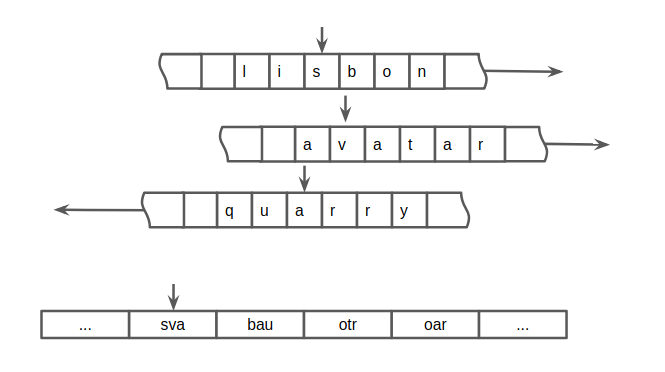
\includegraphics[width=10cm]{ex1.png}
\caption{Simulating a machine $M$ with three tapes using a machine $\widetilde{M}$ with a single tape.}
\label{fig:scetch2}
\end{figure}

\begin{figure}[!ht]
\centering
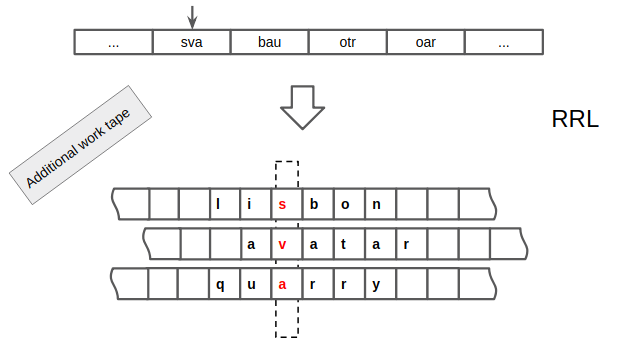
\includegraphics[width=10cm]{ex2.png}
\caption{Simulating a machine $M$ with three tapes using a machine $\widetilde{M}$ with a single tape.}
\label{fig:scetch2}
\end{figure}

\begin{figure}[!ht]
\centering
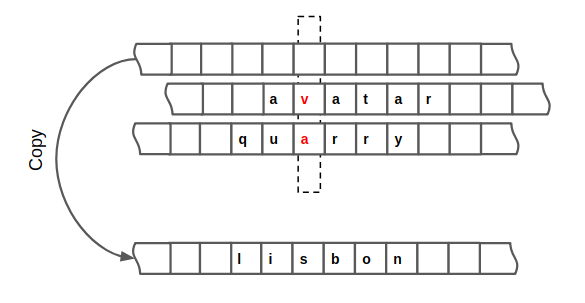
\includegraphics[width=10cm]{ex3.png}
\caption{Simulating a machine $M$ with three tapes using a machine $\widetilde{M}$ with a single tape.}
\label{fig:scetch2}
\end{figure}

\begin{figure}[!ht]
\centering
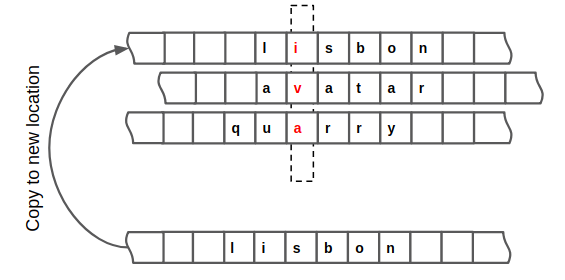
\includegraphics[width=10cm]{ex4.png}
\caption{Simulating a machine $M$ with three tapes using a machine $\widetilde{M}$ with a single tape.}
\label{fig:scetch2}
\end{figure}

\begin{figure}[!ht]
\centering
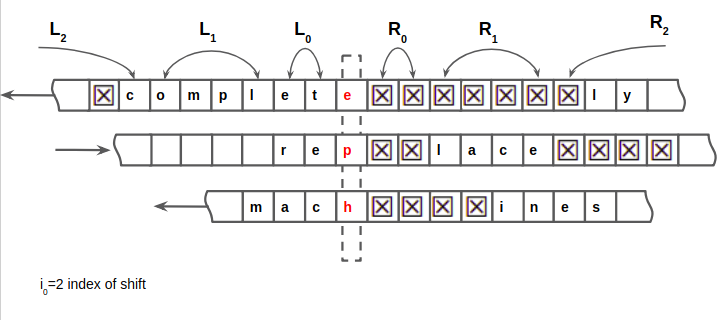
\includegraphics[width=10cm]{al1.png}
\caption{Simulating a machine $M$ with three tapes using a machine $\widetilde{M}$ with a single tape.}
\label{fig:scetch2}
\end{figure}

\begin{figure}[!ht]
\centering
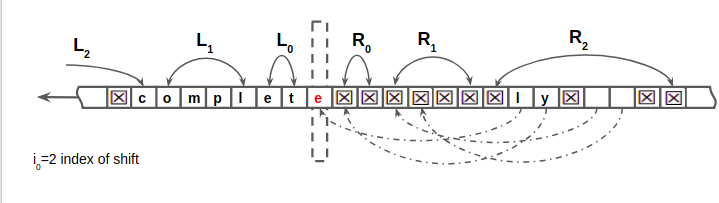
\includegraphics[width=10cm]{al2.png}
\caption{Simulating a machine $M$ with three tapes using a machine $\widetilde{M}$ with a single tape.}
\label{fig:scetch2}
\end{figure}

\begin{figure}[!ht]
\centering
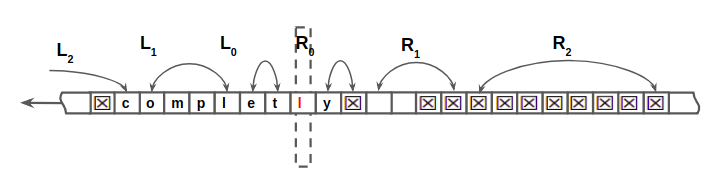
\includegraphics[width=10cm]{al3.png}
\caption{Simulating a machine $M$ with three tapes using a machine $\widetilde{M}$ with a single tape.}
\label{fig:scetch2}
\end{figure}

\begin{figure}[!ht]
\centering
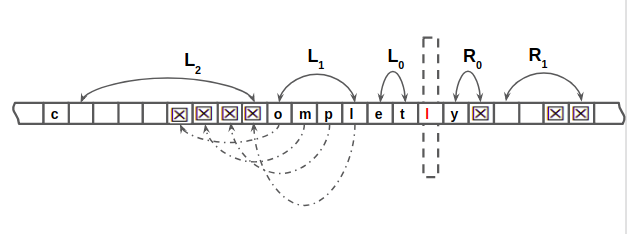
\includegraphics[width=10cm]{al4.png}
\caption{Simulating a machine $M$ with three tapes using a machine $\widetilde{M}$ with a single tape.}
\label{fig:scetch2}
\end{figure}

\begin{figure}[!ht]
\centering
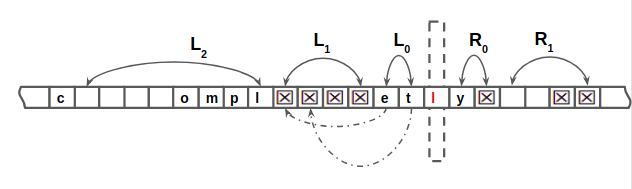
\includegraphics[width=10cm]{al5.png}
\caption{Simulating a machine $M$ with three tapes using a machine $\widetilde{M}$ with a single tape.}
\label{fig:scetch2}
\end{figure}

\begin{figure}[!ht]
\centering
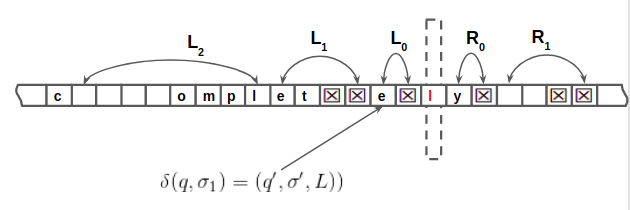
\includegraphics[width=10cm]{al6.png}
\caption{Simulating a machine $M$ with three tapes using a machine $\widetilde{M}$ with a single tape.}
\label{fig:scetch2}
\end{figure}

\begin{figure}[!ht]
\centering
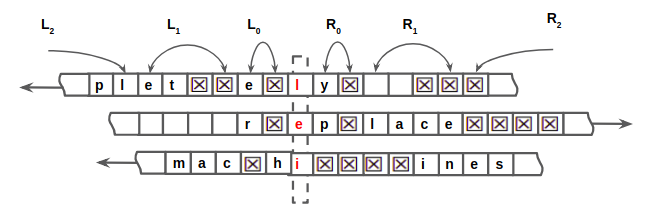
\includegraphics[width=10cm]{al7.png}
\caption{Simulating a machine $M$ with three tapes using a machine $\widetilde{M}$ with a single tape.}
\label{fig:scetch2}
\end{figure}


\end{document}